We used a number of tests to validate the code: unit testing, integration testing, and system testing. There are unit tests that test each individual function in the code. For integration testing, we selected a suite of simple problems all using a single material on a square domain for which we could derive or approximate analytic solutions. We varied the material properties to trigger use of the various solvers. The integration problems used a single energy group with no scattering, a single energy group with scattering, and two energy groups with scattering, respectively. 
% are the details of these tests available somewhere? In a repo you can point to? For reproducibility and reader completeness we need to be able to find the actual details. 

\section{NDA/SAAF Agreement}
% we need a problem description here. 

We also tested the agreement between the NDA+SAAF and SAAF alone to ensure we were replicating expected behavior. As the SAAF equation is non-conservative, its solution does not necessarily agree with the low-order equation with which it is coupled. However, the two solutions should approach each other as the number of mesh cells increases \cite{Wang2013}. We checked if our code replicated this behavior in a number of ways. First, we simply compare the mean difference in the SAAF and NDA scalar fluxes as the number of mesh cells increases. We notice a consistent rate of convergence as seen in Figure~\ref{fig:SAAFvsNDA}. 
%
\begin{figure}[H]
    \centering
    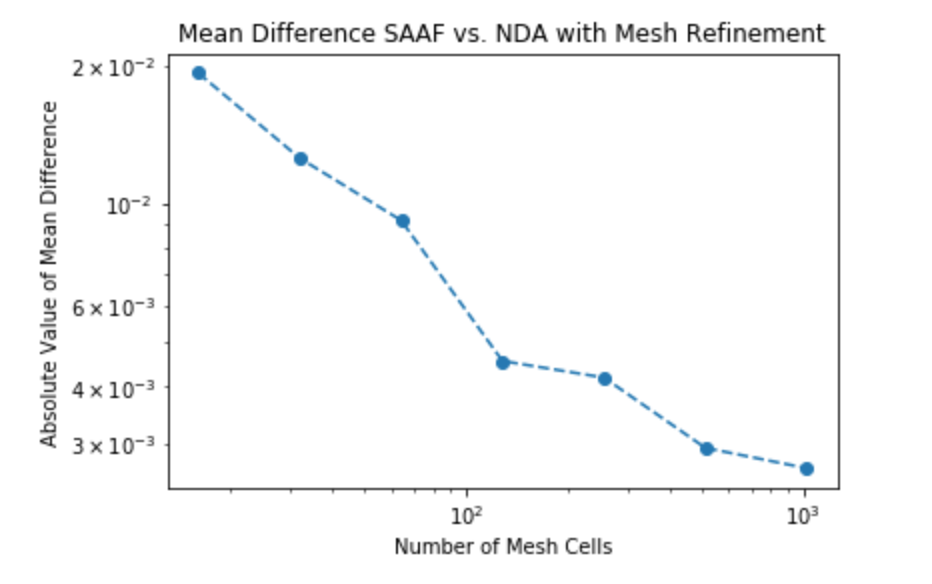
\includegraphics[width=.75\textwidth]{fig/NDAvsSAAF.png}
    \caption{Comparison of SAAF and NDA Scalar Flux with Mesh Refinement for PROBLEM}
    \label{fig:SAAFvsNDA}
\end{figure}

Second, we look at the error in the absorption rate, $\int_\mathcal{D}\Sigma_a\phi$,
% you should probably tell us what D is
 using the NDA solution with a fine-mesh SAAF solution taken as the reference. The difference steadily decreases as the number of mesh cells increase.
%
\begin{figure}[H]
    \centering
    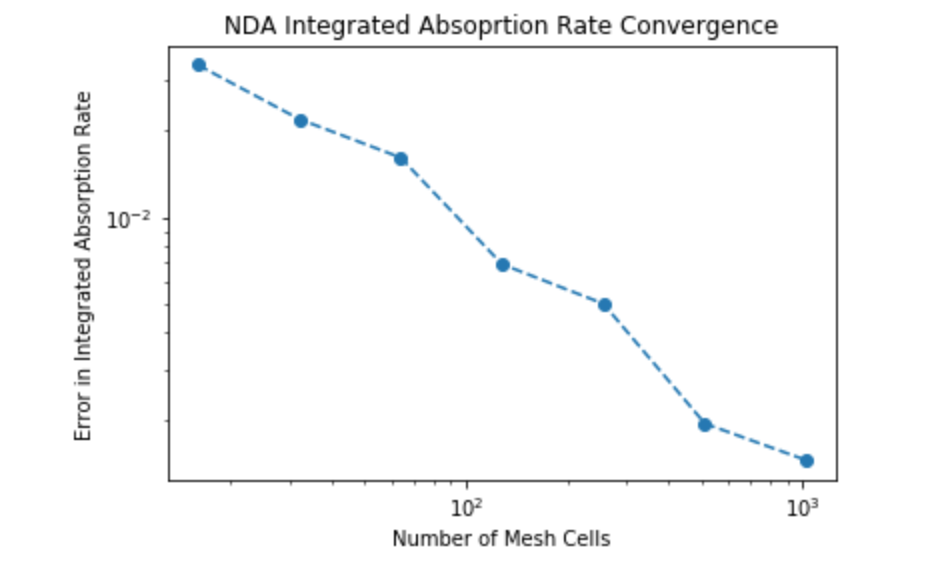
\includegraphics[width=.75\textwidth]{fig/NDAAbsorptionLogLog.png}
    \caption{Error in NDA Absorption Rate as Mesh Refines for PROBLEM}
    \label{fig:abs_err}
\end{figure}
% So here, you're showing the NDA solution converges towards the SAAF solution taken as a reference, where the first problem you're showing they become close together as you refine the mesh of each? You might want to make that a little clearer.

Finally, we chose one test material with one group and some scattering. The purpose of this test is to confirm NDA-SAAF and SAAF match one another, and to see how they compare to diffusion alone. We looked at the scalar flux along the x-direction at \textbf{some location in the problem} from the diffusion equation alone, SAAF with NDA, and SAAF alone. As shown in Figure~\ref{fig:comparison}, we can clearly see that NDA has provided a correction to diffusion, producing a solution that is much closer to the higher-order equation than diffusion by itself. 
%
\begin{figure}[H]
    \centering
    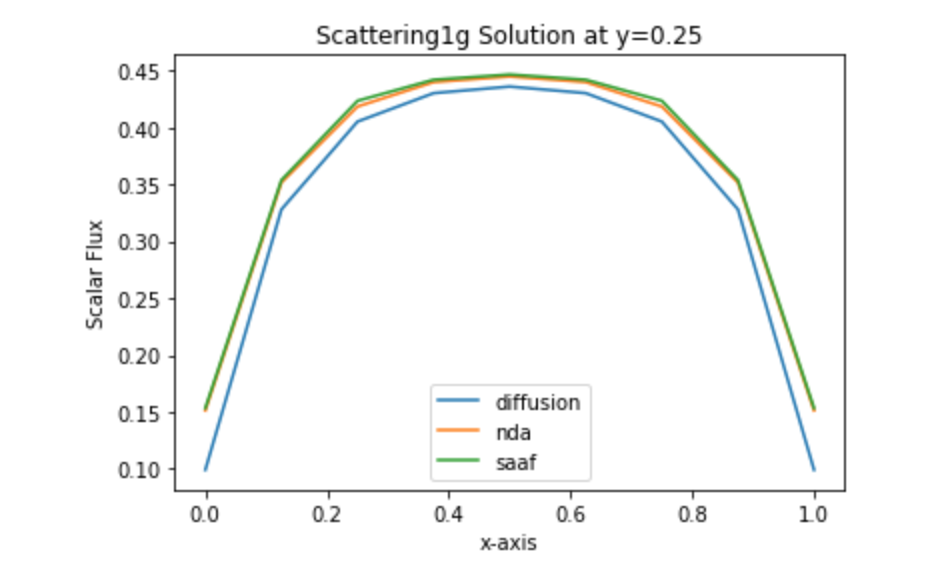
\includegraphics[width=.75\textwidth]{fig/LineOut25.png}
    \caption{Comparison of Diffusion, SAAF, and NDA Scalar Flux for PROBLEM}
    \label{fig:comparison}
\end{figure}

The results of our tests demonstrate the same behavior as previously published work on SAAF+NDA [NEED a REFERENCE]. Therefore, we conclude we have implemented a working version of these methods. 